\scanpage{85}
\mspage{10}
An interesting trivial case is the one where $f$ is an isomorphism --- and even the one where $X=Y$, and where $f$ belongs to a group \inserted{$\mathcal G$} of $K$-isomorphisms of $X$ --- then one can consider $\Pi_1(X)$ and $\Pi_1(X_{\bar K}),\Pi_1(X_K)$ as groupoids on which $\mathcal G$ acts, and $\widehat\Pi_1(X)$ as a groupoid on which $\mathcal G\times\mathbf{\Gamma}$ acts, $\widehat\Pi_1(\bar X_{\bar K})$ as a groupoid on which $\mathcal G\times\Gamma$ acts. This time the group does not act trivially on the vertices of $\Pi_1(X_K)$, the action of $\Gamma$ is trivial, but not necessarily that of $\mathcal G$.

If one is given a point $x_0\in X_K$ as base point, and a set of vertices $I\subset X_K$ containing $x_0$, the action of $\Gamma$ on $\widehat\Pi_1(X,I)$ is known when one \unsure{knows|knows} its action on $\widehat\Pi_1(X,x_0)$, and if moreover one \unsure{knows|knows} its action on the $\widehat\Pi_1(X,x_0)$-torsors ! right
\figure{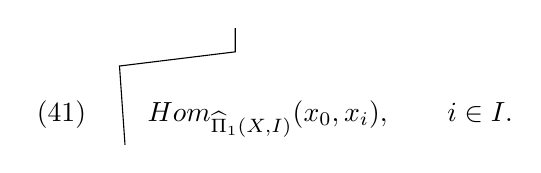
\begin{tikzpicture}
\node[anchor=base east] at(-.65,0) {$(41)$};
\node[anchor=base west,inner sep=0pt] at(0,0) {$\uline{\operatorname{Hom}}_{\widehat\Pi_1(X,I)}(x_0,x_i),\qquad i\in I.$};
\draw(-.28,-.30)--(-.35,.70)--(1.12,.88)--(1.12,1.18);
\end{tikzpicture}}
or, which amounts to the same, if one knows the
\margin{84}
